\documentclass[conference]{IEEEtran}

\usepackage[dutch]{babel}
\usepackage{multirow}
\usepackage[table,xcdraw]{xcolor}
\usepackage{graphicx}
\usepackage{dblfloatfix}
\usepackage{fixltx2e}



\begin{document}

\title{Project blackjack}

\author{\IEEEauthorblockN{Seyed Kavoos Boloorchi, Daan Flor\'e, Robin Lodrigo en Jonas Wallays}
\IEEEauthorblockA{Hogeschool Gent\\
Bedrijf en organisatie\\
E-mail: seyedkavoos.boloorchi.u1660@student.hogent.be,
daan.flore.u8852@student.hogent.be,\\
robin.lodrigo.u8341@student.hogent.be,
jonas.wallays.u8978@student.hogent.be
}}
\date{April 20, 2015}


\maketitle

\begin{abstract}
Voor het opleidingsonderdeel onderzoekstechnieken in de richting toegepaste informatica aan de Hogeschool Gent, gingen we na of er een manier is om het casino te verslaan bij een spelletje blackjack. Dit onderzochten we door enkele (reeds bestaande) strategie\"{e}n uit te testen en we gingen na hoe we de strategie\"{e}n kunnen verbeteren.
\end{abstract}

\IEEEpeerreviewmaketitle

\section{Introductie}
Sinds het ontstaan van blackjack is er reeds veel onderzoek verricht naar een ultieme strategie waarmee men het spelletje zo goed als altijd zou kunnen winnen. Het grootste deel van deze onderzoeken stellen voorop dat deze strategie niet zou bestaan. Er bestaan wel andere strategie\"{e}n die de kans op winst zouden verhogen. Hiervan zijn de basic en perfect strategie ongetwijfeld de meest gekende. We besloten deze twee strategie\"{e}n te vergelijken door gebruik te maken van simulators. Dit doen we door aanvankelijk 1000 handen van blackjack te spelen door willekeurig gegenereerde spelers. We probeerden deze strategie\"{e}n ook aan te passen zodat, statistisch gezien, de winst verhoogt. 

\section{Strategie met de meeste kans op winst}
\subsection{Onderzochte strategie\"{e}n}
Voor dit onderzoek werkten we met de basic en de perfect strategie.
\subsubsection{Basic strategie}
De basic strategie - de meest algemene en gebruikte strategie - is ontstaan door een computer miljoenen simulaties van het spel te laten spelen. Hieruit kon men concluderen wat een speler in het algemeen het best zou doen in verschillende situaties. De resultaten zijn gebaseerd op de kaarten die de dealer toont en de kaarten die de speler heeft. Dit resulteerde in de basic strategy card. Deze strategie is de eerste die wordt geleerd wanneer men professioneel blackjack gaat spelen

\subsubsection{Perfect strategie}
De perfect strategie wordt gebruikt door iets meer ervaren spelers, en is een uitbreiding/aanpassing van de basic strategie.

\subsection{Strategie\"{e}n in de praktijk}
De basic strategie houdt rekening met het totaal van de kaarten die de dealer heeft omgedraaid en het totaal van de kaarten van de speler. Zo moet men in de praktijk op bepaalde situaties verschillend reageren, zoals weergegeven in onderstaande tabellen.




\begin{table}[htbp]
\setlength{\tabcolsep}{3pt}
\caption{Basic strategie}
\tiny
\centering
\begin{tabular}{|c|c|c|c|c|c|c|c|c|c|c|}
\hline
 & \multicolumn{10}{c|}{\textbf{Dealer's face-up card}} \\ \cline{2-11} 
\multirow{-2}{*}{\textbf{\begin{tabular}[c]{@{}c@{}}Player\\ hand\end{tabular}}} & \textbf{2} & \textbf{3} & \textbf{4} & \textbf{5} & \textbf{6} & \textbf{7} & \textbf{8} & \textbf{9} & \textbf{10} & \textbf{11} \\ \hline
\multicolumn{11}{|c|}{\textbf{Hard totals (excluding pairs)}} \\ \hline
\textbf{21} & \cellcolor[HTML]{32CB00}S & \cellcolor[HTML]{32CB00}S & \cellcolor[HTML]{32CB00}S & \cellcolor[HTML]{32CB00}S & \cellcolor[HTML]{32CB00}S & \cellcolor[HTML]{32CB00}S & \cellcolor[HTML]{32CB00}S & \cellcolor[HTML]{32CB00}S & \cellcolor[HTML]{32CB00}S & \cellcolor[HTML]{32CB00}S \\ \hline
\textbf{20} & \cellcolor[HTML]{32CB00}S & \cellcolor[HTML]{32CB00}S & \cellcolor[HTML]{32CB00}S & \cellcolor[HTML]{32CB00}S & \cellcolor[HTML]{32CB00}S & \cellcolor[HTML]{32CB00}S & \cellcolor[HTML]{32CB00}S & \cellcolor[HTML]{32CB00}S & \cellcolor[HTML]{32CB00}S & \cellcolor[HTML]{32CB00}S \\ \hline
\textbf{19} & \cellcolor[HTML]{32CB00}S & \cellcolor[HTML]{32CB00}S & \cellcolor[HTML]{32CB00}S & \cellcolor[HTML]{32CB00}S & \cellcolor[HTML]{32CB00}S & \cellcolor[HTML]{32CB00}S & \cellcolor[HTML]{32CB00}S & \cellcolor[HTML]{32CB00}S & \cellcolor[HTML]{32CB00}S & \cellcolor[HTML]{32CB00}S \\ \hline
\textbf{18} & \cellcolor[HTML]{32CB00}S & \cellcolor[HTML]{32CB00}S & \cellcolor[HTML]{32CB00}S & \cellcolor[HTML]{32CB00}S & \cellcolor[HTML]{32CB00}S & \cellcolor[HTML]{32CB00}S & \cellcolor[HTML]{32CB00}S & \cellcolor[HTML]{32CB00}S & \cellcolor[HTML]{32CB00}S & \cellcolor[HTML]{32CB00}S \\ \hline
\textbf{17} & \cellcolor[HTML]{32CB00}S & \cellcolor[HTML]{32CB00}S & \cellcolor[HTML]{32CB00}S & \cellcolor[HTML]{32CB00}S & \cellcolor[HTML]{32CB00}S & \cellcolor[HTML]{32CB00}S & \cellcolor[HTML]{32CB00}S & \cellcolor[HTML]{32CB00}S & \cellcolor[HTML]{32CB00}S & \cellcolor[HTML]{32CB00}S \\ \hline
\textbf{16} & \cellcolor[HTML]{32CB00}S & \cellcolor[HTML]{32CB00}S & \cellcolor[HTML]{32CB00}S & \cellcolor[HTML]{32CB00}S & \cellcolor[HTML]{32CB00}S & \cellcolor[HTML]{FE0000}H & \cellcolor[HTML]{FE0000}H & \cellcolor[HTML]{34CDF9}SU/H & \cellcolor[HTML]{34CDF9}SU/H & \cellcolor[HTML]{34CDF9}SU/H \\ \hline
\textbf{15} & \cellcolor[HTML]{32CB00}S & \cellcolor[HTML]{32CB00}S & \cellcolor[HTML]{32CB00}S & \cellcolor[HTML]{32CB00}S & \cellcolor[HTML]{32CB00}S & \cellcolor[HTML]{FE0000}H & \cellcolor[HTML]{FE0000}H & \cellcolor[HTML]{FE0000}H & \cellcolor[HTML]{34CDF9}SU/H & \cellcolor[HTML]{FE0000}H \\ \hline
\textbf{14} & \cellcolor[HTML]{32CB00}S & \cellcolor[HTML]{32CB00}S & \cellcolor[HTML]{32CB00}S & \cellcolor[HTML]{32CB00}S & \cellcolor[HTML]{32CB00}S & \cellcolor[HTML]{FE0000}H & \cellcolor[HTML]{FE0000}H & \cellcolor[HTML]{FE0000}H & \cellcolor[HTML]{FE0000}H & \cellcolor[HTML]{FE0000}H \\ \hline
\textbf{13} & \cellcolor[HTML]{32CB00}S & \cellcolor[HTML]{32CB00}S & \cellcolor[HTML]{32CB00}S & \cellcolor[HTML]{32CB00}S & \cellcolor[HTML]{32CB00}S & \cellcolor[HTML]{FE0000}H & \cellcolor[HTML]{FE0000}H & \cellcolor[HTML]{FE0000}H & \cellcolor[HTML]{FE0000}H & \cellcolor[HTML]{FE0000}H \\ \hline
\textbf{12} & \cellcolor[HTML]{FE0000}H & \cellcolor[HTML]{FE0000}H & \cellcolor[HTML]{32CB00}S & \cellcolor[HTML]{32CB00}S & \cellcolor[HTML]{32CB00}S & \cellcolor[HTML]{FE0000}H & \cellcolor[HTML]{FE0000}H & \cellcolor[HTML]{FE0000}H & \cellcolor[HTML]{FE0000}H & \cellcolor[HTML]{FE0000}H \\ \hline
\textbf{11} & \cellcolor[HTML]{FFC702}D/H & \cellcolor[HTML]{FFC702}D/H & \cellcolor[HTML]{FFC702}D/H & \cellcolor[HTML]{FFC702}D/H & \cellcolor[HTML]{FFC702}D/H & \cellcolor[HTML]{FFC702}D/H & \cellcolor[HTML]{FFC702}D/H & \cellcolor[HTML]{FFC702}D/H & \cellcolor[HTML]{FFC702}D/H & \cellcolor[HTML]{FE0000}H \\ \hline
\textbf{10} & \cellcolor[HTML]{FFC702}D/H & \cellcolor[HTML]{FFC702}D/H & \cellcolor[HTML]{FFC702}D/H & \cellcolor[HTML]{FFC702}D/H & \cellcolor[HTML]{FFC702}D/H & \cellcolor[HTML]{FFC702}D/H & \cellcolor[HTML]{FFC702}D/H & \cellcolor[HTML]{FFC702}D/H & \cellcolor[HTML]{FE0000}H & \cellcolor[HTML]{FE0000}H \\ \hline
\textbf{9} & \cellcolor[HTML]{FE0000}H & \cellcolor[HTML]{FFC702}D/H & \cellcolor[HTML]{FFC702}D/H & \cellcolor[HTML]{FFC702}D/H & \cellcolor[HTML]{FFC702}D/H & \cellcolor[HTML]{FE0000}H & \cellcolor[HTML]{FE0000}H & \cellcolor[HTML]{FE0000}H & \cellcolor[HTML]{FE0000}H & \cellcolor[HTML]{FE0000}H \\ \hline
\textbf{8} & \cellcolor[HTML]{FE0000}H & \cellcolor[HTML]{FE0000}H & \cellcolor[HTML]{FE0000}H & \cellcolor[HTML]{FE0000}H & \cellcolor[HTML]{FE0000}H & \cellcolor[HTML]{FE0000}H & \cellcolor[HTML]{FE0000}H & \cellcolor[HTML]{FE0000}H & \cellcolor[HTML]{FE0000}H & \cellcolor[HTML]{FE0000}H \\ \hline
\textbf{7} & \cellcolor[HTML]{FE0000}H & \cellcolor[HTML]{FE0000}H & \cellcolor[HTML]{FE0000}H & \cellcolor[HTML]{FE0000}H & \cellcolor[HTML]{FE0000}H & \cellcolor[HTML]{FE0000}H & \cellcolor[HTML]{FE0000}H & \cellcolor[HTML]{FE0000}H & \cellcolor[HTML]{FE0000}H & \cellcolor[HTML]{FE0000}H \\ \hline
\textbf{6} & \cellcolor[HTML]{FE0000}H & \cellcolor[HTML]{FE0000}H & \cellcolor[HTML]{FE0000}H & \cellcolor[HTML]{FE0000}H & \cellcolor[HTML]{FE0000}H & \cellcolor[HTML]{FE0000}H & \cellcolor[HTML]{FE0000}H & \cellcolor[HTML]{FE0000}H & \cellcolor[HTML]{FE0000}H & \cellcolor[HTML]{FE0000}H \\ \hline
\textbf{5} & \cellcolor[HTML]{FE0000}H & \cellcolor[HTML]{FE0000}H & \cellcolor[HTML]{FE0000}H & \cellcolor[HTML]{FE0000}H & \cellcolor[HTML]{FE0000}H & \cellcolor[HTML]{FE0000}H & \cellcolor[HTML]{FE0000}H & \cellcolor[HTML]{FE0000}H & \cellcolor[HTML]{FE0000}H & \cellcolor[HTML]{FE0000}H \\ \hline
\multicolumn{11}{|c|}{\textbf{Soft totals}} \\ \hline
\textbf{21} & \cellcolor[HTML]{32CB00}S & \cellcolor[HTML]{32CB00}S & \cellcolor[HTML]{32CB00}S & \cellcolor[HTML]{32CB00}S & \cellcolor[HTML]{32CB00}S & \cellcolor[HTML]{32CB00}S & \cellcolor[HTML]{32CB00}S & \cellcolor[HTML]{32CB00}S & \cellcolor[HTML]{32CB00}S & \cellcolor[HTML]{32CB00}S \\ \hline
\textbf{20} & \cellcolor[HTML]{32CB00}S & \cellcolor[HTML]{32CB00}S & \cellcolor[HTML]{32CB00}S & \cellcolor[HTML]{32CB00}S & \cellcolor[HTML]{32CB00}S & \cellcolor[HTML]{32CB00}S & \cellcolor[HTML]{32CB00}S & \cellcolor[HTML]{32CB00}S & \cellcolor[HTML]{32CB00}S & \cellcolor[HTML]{32CB00}S \\ \hline
\textbf{19} & \cellcolor[HTML]{32CB00}S & \cellcolor[HTML]{32CB00}S & \cellcolor[HTML]{32CB00}S & \cellcolor[HTML]{32CB00}S & \cellcolor[HTML]{32CB00}S & \cellcolor[HTML]{32CB00}S & \cellcolor[HTML]{32CB00}S & \cellcolor[HTML]{32CB00}S & \cellcolor[HTML]{32CB00}S & \cellcolor[HTML]{32CB00}S \\ \hline
\textbf{18} & \cellcolor[HTML]{32CB00}S & \cellcolor[HTML]{FFC702}D/S & \cellcolor[HTML]{FFC702}D/S & \cellcolor[HTML]{FFC702}D/S & \cellcolor[HTML]{FFC702}D/S & \cellcolor[HTML]{32CB00}S & \cellcolor[HTML]{32CB00}S & \cellcolor[HTML]{FE0000}H & \cellcolor[HTML]{FE0000}H & \cellcolor[HTML]{FE0000}H \\ \hline
\textbf{17} & \cellcolor[HTML]{FE0000}H & \cellcolor[HTML]{FFC702}D/H & \cellcolor[HTML]{FFC702}D/H & \cellcolor[HTML]{FFC702}D/H & \cellcolor[HTML]{FFC702}D/H & \cellcolor[HTML]{FE0000}H & \cellcolor[HTML]{FE0000}H & \cellcolor[HTML]{FE0000}H & \cellcolor[HTML]{FE0000}H & \cellcolor[HTML]{FE0000}H \\ \hline
\textbf{16} & \cellcolor[HTML]{FE0000}H & \cellcolor[HTML]{FE0000}H & \cellcolor[HTML]{FFC702}D/H & \cellcolor[HTML]{FFC702}D/H & \cellcolor[HTML]{FFC702}D/H & \cellcolor[HTML]{FE0000}H & \cellcolor[HTML]{FE0000}H & \cellcolor[HTML]{FE0000}H & \cellcolor[HTML]{FE0000}H & \cellcolor[HTML]{FE0000}H \\ \hline
\textbf{15} & \cellcolor[HTML]{FE0000}H & \cellcolor[HTML]{FE0000}H & \cellcolor[HTML]{FFC702}D/H & \cellcolor[HTML]{FFC702}D/H & \cellcolor[HTML]{FFC702}D/H & \cellcolor[HTML]{FE0000}H & \cellcolor[HTML]{FE0000}H & \cellcolor[HTML]{FE0000}H & \cellcolor[HTML]{FE0000}H & \cellcolor[HTML]{FE0000}H \\ \hline
\textbf{14} & \cellcolor[HTML]{FE0000}H & \cellcolor[HTML]{FE0000}H & \cellcolor[HTML]{FE0000}H & \cellcolor[HTML]{FFC702}D/H & \cellcolor[HTML]{FFC702}D/H & \cellcolor[HTML]{FE0000}H & \cellcolor[HTML]{FE0000}H & \cellcolor[HTML]{FE0000}H & \cellcolor[HTML]{FE0000}H & \cellcolor[HTML]{FE0000}H \\ \hline
\textbf{13} & \cellcolor[HTML]{FE0000}H & \cellcolor[HTML]{FE0000}H & \cellcolor[HTML]{FE0000}H & \cellcolor[HTML]{FFC702}D/H & \cellcolor[HTML]{FFC702}D/H & \cellcolor[HTML]{FE0000}H & \cellcolor[HTML]{FE0000}H & \cellcolor[HTML]{FE0000}H & \cellcolor[HTML]{FE0000}H & \cellcolor[HTML]{FE0000}H \\ \hline
\multicolumn{11}{|c|}{\textbf{Pairs}} \\ \hline
\textbf{A,A} & \cellcolor[HTML]{F8FF00}SP/H & \cellcolor[HTML]{F8FF00}SP/H & \cellcolor[HTML]{F8FF00}SP/H & \cellcolor[HTML]{F8FF00}SP/H & \cellcolor[HTML]{F8FF00}SP/H & \cellcolor[HTML]{F8FF00}SP/H & \cellcolor[HTML]{F8FF00}SP/H & \cellcolor[HTML]{F8FF00}SP/H & \cellcolor[HTML]{F8FF00}SP/H & \cellcolor[HTML]{F8FF00}SP/H \\ \hline
\textbf{20} & \cellcolor[HTML]{32CB00}S & \cellcolor[HTML]{32CB00}S & \cellcolor[HTML]{32CB00}S & \cellcolor[HTML]{32CB00}S & \cellcolor[HTML]{32CB00}S & \cellcolor[HTML]{32CB00}S & \cellcolor[HTML]{32CB00}S & \cellcolor[HTML]{32CB00}S & \cellcolor[HTML]{32CB00}S & \cellcolor[HTML]{32CB00}S \\ \hline
\textbf{18} & \cellcolor[HTML]{F8FF00}SP/S & \cellcolor[HTML]{F8FF00}SP/S & \cellcolor[HTML]{F8FF00}SP/S & \cellcolor[HTML]{F8FF00}SP/S & \cellcolor[HTML]{F8FF00}SP/S & \cellcolor[HTML]{32CB00}S & \cellcolor[HTML]{F8FF00}SP/S & \cellcolor[HTML]{F8FF00}SP/S & \cellcolor[HTML]{32CB00}S & \cellcolor[HTML]{32CB00}S \\ \hline
\textbf{16} & \cellcolor[HTML]{F8FF00}SP/S & \cellcolor[HTML]{F8FF00}SP/S & \cellcolor[HTML]{F8FF00}SP/S & \cellcolor[HTML]{F8FF00}SP/S & \cellcolor[HTML]{F8FF00}SP/S & \cellcolor[HTML]{F8FF00}SP/H & \cellcolor[HTML]{F8FF00}SP/H & \cellcolor[HTML]{F8FF00}SP/H & \cellcolor[HTML]{F8FF00}SP/H & \cellcolor[HTML]{F8FF00}SP/H \\ \hline
\textbf{14} & \cellcolor[HTML]{F8FF00}SP/S & \cellcolor[HTML]{F8FF00}SP/S & \cellcolor[HTML]{F8FF00}SP/S & \cellcolor[HTML]{F8FF00}SP/S & \cellcolor[HTML]{F8FF00}SP/S & \cellcolor[HTML]{F8FF00}SP/H & \cellcolor[HTML]{FE0000}H & \cellcolor[HTML]{FE0000}H & \cellcolor[HTML]{FE0000}H & \cellcolor[HTML]{FE0000}H \\ \hline
\textbf{12} & \cellcolor[HTML]{F8FF00}SP/H & \cellcolor[HTML]{F8FF00}SP/H & \cellcolor[HTML]{F8FF00}SP/S & \cellcolor[HTML]{F8FF00}SP/S & \cellcolor[HTML]{F8FF00}SP/S & \cellcolor[HTML]{FE0000}H & \cellcolor[HTML]{FE0000}H & \cellcolor[HTML]{FE0000}H & \cellcolor[HTML]{FE0000}H & \cellcolor[HTML]{FE0000}H \\ \hline
\textbf{10} & \cellcolor[HTML]{FFC702}D/H & \cellcolor[HTML]{FFC702}D/H & \cellcolor[HTML]{FFC702}D/H & \cellcolor[HTML]{FFC702}D/H & \cellcolor[HTML]{FFC702}D/H & \cellcolor[HTML]{FFC702}D/H & \cellcolor[HTML]{FFC702}D/H & \cellcolor[HTML]{FFC702}D/H & \cellcolor[HTML]{FE0000}H & \cellcolor[HTML]{FE0000}H \\ \hline
\textbf{8} & \cellcolor[HTML]{FE0000}H & \cellcolor[HTML]{FE0000}H & \cellcolor[HTML]{FE0000}H & \cellcolor[HTML]{F8FF00}SP/H & \cellcolor[HTML]{F8FF00}SP/H & \cellcolor[HTML]{FE0000}H & \cellcolor[HTML]{FE0000}H & \cellcolor[HTML]{FE0000}H & \cellcolor[HTML]{FE0000}H & \cellcolor[HTML]{FE0000}H \\ \hline
\textbf{6} & \cellcolor[HTML]{F8FF00}SP/H & \cellcolor[HTML]{F8FF00}SP/H & \cellcolor[HTML]{F8FF00}SP/H & \cellcolor[HTML]{F8FF00}SP/H & \cellcolor[HTML]{F8FF00}SP/H & \cellcolor[HTML]{F8FF00}SP/H & \cellcolor[HTML]{FE0000}H & \cellcolor[HTML]{FE0000}H & \cellcolor[HTML]{FE0000}H & \cellcolor[HTML]{FE0000}H \\ \hline
\textbf{4} & \cellcolor[HTML]{F8FF00}SP/H & \cellcolor[HTML]{F8FF00}SP/H & \cellcolor[HTML]{F8FF00}SP/H & \cellcolor[HTML]{F8FF00}SP/H & \cellcolor[HTML]{F8FF00}SP/H & \cellcolor[HTML]{F8FF00}SP/H & \cellcolor[HTML]{FE0000}H & \cellcolor[HTML]{FE0000}H & \cellcolor[HTML]{FE0000}H & \cellcolor[HTML]{FE0000}H \\ \hline
\end{tabular}
\end{table}
\begin{table}[htbp]
\setlength{\tabcolsep}{3pt}
\caption{Perfect strategy}
\tiny
\centering
\begin{tabular}{|c|c|c|c|c|c|c|c|c|c|c|}
\hline
 & \multicolumn{10}{c|}{\textbf{Dealer's face-up card}} \\ \cline{2-11} 
\multirow{-2}{*}{\textbf{\begin{tabular}[c]{@{}c@{}}Player\\ hand\end{tabular}}} & \textbf{2} & \textbf{3} & \textbf{4} & \textbf{5} & \textbf{6} & \textbf{7} & \textbf{8} & \textbf{9} & \textbf{10} & \textbf{11} \\ \hline
\multicolumn{11}{|c|}{\textbf{Hard totals (excluding pairs)}} \\ \hline
\textbf{21} & \cellcolor[HTML]{32CB00}S & \cellcolor[HTML]{32CB00}S & \cellcolor[HTML]{32CB00}S & \cellcolor[HTML]{32CB00}S & \cellcolor[HTML]{32CB00}S & \cellcolor[HTML]{32CB00}S & \cellcolor[HTML]{32CB00}S & \cellcolor[HTML]{32CB00}S & \cellcolor[HTML]{32CB00}S & \cellcolor[HTML]{32CB00}S \\ \hline
\textbf{20} & \cellcolor[HTML]{32CB00}S & \cellcolor[HTML]{32CB00}S & \cellcolor[HTML]{32CB00}S & \cellcolor[HTML]{32CB00}S & \cellcolor[HTML]{32CB00}S & \cellcolor[HTML]{32CB00}S & \cellcolor[HTML]{32CB00}S & \cellcolor[HTML]{32CB00}S & \cellcolor[HTML]{32CB00}S & \cellcolor[HTML]{32CB00}S \\ \hline
\textbf{19} & \cellcolor[HTML]{32CB00}S & \cellcolor[HTML]{32CB00}S & \cellcolor[HTML]{32CB00}S & \cellcolor[HTML]{32CB00}S & \cellcolor[HTML]{32CB00}S & \cellcolor[HTML]{32CB00}S & \cellcolor[HTML]{32CB00}S & \cellcolor[HTML]{32CB00}S & \cellcolor[HTML]{32CB00}S & \cellcolor[HTML]{32CB00}S \\ \hline
\textbf{18} & \cellcolor[HTML]{32CB00}S & \cellcolor[HTML]{32CB00}S & \cellcolor[HTML]{32CB00}S & \cellcolor[HTML]{32CB00}S & \cellcolor[HTML]{32CB00}S & \cellcolor[HTML]{32CB00}S & \cellcolor[HTML]{32CB00}S & \cellcolor[HTML]{32CB00}S & \cellcolor[HTML]{32CB00}S & \cellcolor[HTML]{32CB00}S \\ \hline
\textbf{17} & \cellcolor[HTML]{32CB00}S & \cellcolor[HTML]{32CB00}S & \cellcolor[HTML]{32CB00}S & \cellcolor[HTML]{32CB00}S & \cellcolor[HTML]{32CB00}S & \cellcolor[HTML]{32CB00}S & \cellcolor[HTML]{32CB00}S & \cellcolor[HTML]{32CB00}S & \cellcolor[HTML]{32CB00}S & \cellcolor[HTML]{32CB00}S \\ \hline
\textbf{16} & \cellcolor[HTML]{32CB00}S & \cellcolor[HTML]{32CB00}S & \cellcolor[HTML]{32CB00}S & \cellcolor[HTML]{32CB00}S & \cellcolor[HTML]{32CB00}S & \cellcolor[HTML]{FE0000}H & \cellcolor[HTML]{FE0000}H & \cellcolor[HTML]{FE0000}H & \cellcolor[HTML]{FE0000}H & \cellcolor[HTML]{FE0000}H \\ \hline
\textbf{15} & \cellcolor[HTML]{32CB00}S & \cellcolor[HTML]{32CB00}S & \cellcolor[HTML]{32CB00}S & \cellcolor[HTML]{32CB00}S & \cellcolor[HTML]{32CB00}S & \cellcolor[HTML]{FE0000}H & \cellcolor[HTML]{FE0000}H & \cellcolor[HTML]{FE0000}H & \cellcolor[HTML]{FE0000}H & \cellcolor[HTML]{FE0000}H \\ \hline
\textbf{14} & \cellcolor[HTML]{32CB00}S & \cellcolor[HTML]{32CB00}S & \cellcolor[HTML]{32CB00}S & \cellcolor[HTML]{32CB00}S & \cellcolor[HTML]{32CB00}S & \cellcolor[HTML]{FE0000}H & \cellcolor[HTML]{FE0000}H & \cellcolor[HTML]{FE0000}H & \cellcolor[HTML]{FE0000}H & \cellcolor[HTML]{FE0000}H \\ \hline
\textbf{13} & \cellcolor[HTML]{32CB00}S & \cellcolor[HTML]{32CB00}S & \cellcolor[HTML]{32CB00}S & \cellcolor[HTML]{32CB00}S & \cellcolor[HTML]{32CB00}S & \cellcolor[HTML]{FE0000}H & \cellcolor[HTML]{FE0000}H & \cellcolor[HTML]{FE0000}H & \cellcolor[HTML]{FE0000}H & \cellcolor[HTML]{FE0000}H \\ \hline
\textbf{12} & \cellcolor[HTML]{FE0000}H & \cellcolor[HTML]{FE0000}H & \cellcolor[HTML]{32CB00}S & \cellcolor[HTML]{32CB00}S & \cellcolor[HTML]{32CB00}S & \cellcolor[HTML]{FE0000}H & \cellcolor[HTML]{FE0000}H & \cellcolor[HTML]{FE0000}H & \cellcolor[HTML]{FE0000}H & \cellcolor[HTML]{FE0000}H \\ \hline
\textbf{11} & \cellcolor[HTML]{FFC702}D/H & \cellcolor[HTML]{FFC702}D/H & \cellcolor[HTML]{FFC702}D/H & \cellcolor[HTML]{FFC702}D/H & \cellcolor[HTML]{FFC702}D/H & \cellcolor[HTML]{FFC702}D/H & \cellcolor[HTML]{FFC702}D/H & \cellcolor[HTML]{FFC702}D/H & \cellcolor[HTML]{FFC702}D/H & \cellcolor[HTML]{FE0000}H \\ \hline
\textbf{10} & \cellcolor[HTML]{FFC702}D/H & \cellcolor[HTML]{FFC702}D/H & \cellcolor[HTML]{FFC702}D/H & \cellcolor[HTML]{FFC702}D/H & \cellcolor[HTML]{FFC702}D/H & \cellcolor[HTML]{FFC702}D/H & \cellcolor[HTML]{FFC702}D/H & \cellcolor[HTML]{FFC702}D/H & \cellcolor[HTML]{FE0000}H & \cellcolor[HTML]{FE0000}H \\ \hline
\textbf{9} & \cellcolor[HTML]{FE0000}H & \cellcolor[HTML]{FFC702}D/H & \cellcolor[HTML]{FFC702}D/H & \cellcolor[HTML]{FFC702}D/H & \cellcolor[HTML]{FFC702}D/H & \cellcolor[HTML]{FE0000}H & \cellcolor[HTML]{FE0000}H & \cellcolor[HTML]{FE0000}H & \cellcolor[HTML]{FE0000}H & \cellcolor[HTML]{FE0000}H \\ \hline
\textbf{8} & \cellcolor[HTML]{FE0000}H & \cellcolor[HTML]{FE0000}H & \cellcolor[HTML]{FE0000}H & \cellcolor[HTML]{FE0000}H & \cellcolor[HTML]{FE0000}H & \cellcolor[HTML]{FE0000}H & \cellcolor[HTML]{FE0000}H & \cellcolor[HTML]{FE0000}H & \cellcolor[HTML]{FE0000}H & \cellcolor[HTML]{FE0000}H \\ \hline
\textbf{7} & \cellcolor[HTML]{FE0000}H & \cellcolor[HTML]{FE0000}H & \cellcolor[HTML]{FE0000}H & \cellcolor[HTML]{FE0000}H & \cellcolor[HTML]{FE0000}H & \cellcolor[HTML]{FE0000}H & \cellcolor[HTML]{FE0000}H & \cellcolor[HTML]{FE0000}H & \cellcolor[HTML]{FE0000}H & \cellcolor[HTML]{FE0000}H \\ \hline
\textbf{6} & \cellcolor[HTML]{FE0000}H & \cellcolor[HTML]{FE0000}H & \cellcolor[HTML]{FE0000}H & \cellcolor[HTML]{FE0000}H & \cellcolor[HTML]{FE0000}H & \cellcolor[HTML]{FE0000}H & \cellcolor[HTML]{FE0000}H & \cellcolor[HTML]{FE0000}H & \cellcolor[HTML]{FE0000}H & \cellcolor[HTML]{FE0000}H \\ \hline
\textbf{5} & \cellcolor[HTML]{FE0000}H & \cellcolor[HTML]{FE0000}H & \cellcolor[HTML]{FE0000}H & \cellcolor[HTML]{FE0000}H & \cellcolor[HTML]{FE0000}H & \cellcolor[HTML]{FE0000}H & \cellcolor[HTML]{FE0000}H & \cellcolor[HTML]{FE0000}H & \cellcolor[HTML]{FE0000}H & \cellcolor[HTML]{FE0000}H \\ \hline
\multicolumn{11}{|c|}{\textbf{Soft totals}} \\ \hline
\textbf{21} & \cellcolor[HTML]{32CB00}S & \cellcolor[HTML]{32CB00}S & \cellcolor[HTML]{32CB00}S & \cellcolor[HTML]{32CB00}S & \cellcolor[HTML]{32CB00}S & \cellcolor[HTML]{32CB00}S & \cellcolor[HTML]{32CB00}S & \cellcolor[HTML]{32CB00}S & \cellcolor[HTML]{32CB00}S & \cellcolor[HTML]{32CB00}S \\ \hline
\textbf{20} & \cellcolor[HTML]{32CB00}S & \cellcolor[HTML]{32CB00}S & \cellcolor[HTML]{32CB00}S & \cellcolor[HTML]{32CB00}S & \cellcolor[HTML]{32CB00}S & \cellcolor[HTML]{32CB00}S & \cellcolor[HTML]{32CB00}S & \cellcolor[HTML]{32CB00}S & \cellcolor[HTML]{32CB00}S & \cellcolor[HTML]{32CB00}S \\ \hline
\textbf{19} & \cellcolor[HTML]{32CB00}S & \cellcolor[HTML]{32CB00}S & \cellcolor[HTML]{32CB00}S & \cellcolor[HTML]{32CB00}S & \cellcolor[HTML]{32CB00}S & \cellcolor[HTML]{32CB00}S & \cellcolor[HTML]{32CB00}S & \cellcolor[HTML]{32CB00}S & \cellcolor[HTML]{32CB00}S & \cellcolor[HTML]{32CB00}S \\ \hline
\textbf{18} & \cellcolor[HTML]{32CB00}S & \cellcolor[HTML]{32CB00}S & \cellcolor[HTML]{32CB00}S & \cellcolor[HTML]{32CB00}S & \cellcolor[HTML]{FFC702}D/S & \cellcolor[HTML]{32CB00}S & \cellcolor[HTML]{32CB00}S & \cellcolor[HTML]{FE0000}H & \cellcolor[HTML]{FE0000}H & \cellcolor[HTML]{FE0000}H \\ \hline
\textbf{17} & \cellcolor[HTML]{FE0000}H & \cellcolor[HTML]{FFC702}D/H & \cellcolor[HTML]{FFC702}D/H & \cellcolor[HTML]{FFC702}D/H & \cellcolor[HTML]{FFC702}D/H & \cellcolor[HTML]{FE0000}H & \cellcolor[HTML]{FE0000}H & \cellcolor[HTML]{FE0000}H & \cellcolor[HTML]{FE0000}H & \cellcolor[HTML]{FE0000}H \\ \hline
\textbf{16} & \cellcolor[HTML]{FE0000}H & \cellcolor[HTML]{FE0000}H & \cellcolor[HTML]{FFC702}D/H & \cellcolor[HTML]{FFC702}D/H & \cellcolor[HTML]{FFC702}D/H & \cellcolor[HTML]{FE0000}H & \cellcolor[HTML]{FE0000}H & \cellcolor[HTML]{FE0000}H & \cellcolor[HTML]{FE0000}H & \cellcolor[HTML]{FE0000}H \\ \hline
\textbf{15} & \cellcolor[HTML]{FE0000}H & \cellcolor[HTML]{FE0000}H & \cellcolor[HTML]{FFC702}D/H & \cellcolor[HTML]{FFC702}D/H & \cellcolor[HTML]{FFC702}D/H & \cellcolor[HTML]{FE0000}H & \cellcolor[HTML]{FE0000}H & \cellcolor[HTML]{FE0000}H & \cellcolor[HTML]{FE0000}H & \cellcolor[HTML]{FE0000}H \\ \hline
\textbf{14} & \cellcolor[HTML]{FE0000}H & \cellcolor[HTML]{FE0000}H & \cellcolor[HTML]{FE0000}H & \cellcolor[HTML]{FFC702}D/H & \cellcolor[HTML]{FFC702}D/H & \cellcolor[HTML]{FE0000}H & \cellcolor[HTML]{FE0000}H & \cellcolor[HTML]{FE0000}H & \cellcolor[HTML]{FE0000}H & \cellcolor[HTML]{FE0000}H \\ \hline
\textbf{13} & \cellcolor[HTML]{FE0000}H & \cellcolor[HTML]{FE0000}H & \cellcolor[HTML]{FE0000}H & \cellcolor[HTML]{FFC702}D/H & \cellcolor[HTML]{FFC702}D/H & \cellcolor[HTML]{FE0000}H & \cellcolor[HTML]{FE0000}H & \cellcolor[HTML]{FE0000}H & \cellcolor[HTML]{FE0000}H & \cellcolor[HTML]{FE0000}H \\ \hline
\multicolumn{11}{|c|}{\textbf{Pairs}} \\ \hline
\textbf{A,A} & \cellcolor[HTML]{F8FF00}SP/H & \cellcolor[HTML]{F8FF00}SP/H & \cellcolor[HTML]{F8FF00}SP/H & \cellcolor[HTML]{F8FF00}SP/H & \cellcolor[HTML]{F8FF00}SP/H & \cellcolor[HTML]{F8FF00}SP/H & \cellcolor[HTML]{F8FF00}SP/H & \cellcolor[HTML]{F8FF00}SP/H & \cellcolor[HTML]{F8FF00}SP/H & \cellcolor[HTML]{F8FF00}SP/H \\ \hline
\textbf{20} & \cellcolor[HTML]{32CB00}S & \cellcolor[HTML]{32CB00}S & \cellcolor[HTML]{32CB00}S & \cellcolor[HTML]{32CB00}S & \cellcolor[HTML]{32CB00}S & \cellcolor[HTML]{32CB00}S & \cellcolor[HTML]{32CB00}S & \cellcolor[HTML]{32CB00}S & \cellcolor[HTML]{32CB00}S & \cellcolor[HTML]{32CB00}S \\ \hline
\textbf{18} & \cellcolor[HTML]{F8FF00}SP/S & \cellcolor[HTML]{F8FF00}SP/S & \cellcolor[HTML]{F8FF00}SP/S & \cellcolor[HTML]{F8FF00}SP/S & \cellcolor[HTML]{F8FF00}SP/S & \cellcolor[HTML]{32CB00}S & \cellcolor[HTML]{F8FF00}SP/S & \cellcolor[HTML]{F8FF00}SP/S & \cellcolor[HTML]{32CB00}S & \cellcolor[HTML]{32CB00}S \\ \hline
\textbf{16} & \cellcolor[HTML]{F8FF00}SP/S & \cellcolor[HTML]{F8FF00}SP/S & \cellcolor[HTML]{F8FF00}SP/S & \cellcolor[HTML]{F8FF00}SP/S & \cellcolor[HTML]{F8FF00}SP/S & \cellcolor[HTML]{F8FF00}SP/H & \cellcolor[HTML]{F8FF00}SP/H & \cellcolor[HTML]{F8FF00}SP/H & \cellcolor[HTML]{F8FF00}SP/H & \cellcolor[HTML]{F8FF00}SP/H \\ \hline
\textbf{14} & \cellcolor[HTML]{F8FF00}SP/S & \cellcolor[HTML]{F8FF00}SP/S & \cellcolor[HTML]{F8FF00}SP/S & \cellcolor[HTML]{F8FF00}SP/S & \cellcolor[HTML]{F8FF00}SP/S & \cellcolor[HTML]{F8FF00}SP/H & \cellcolor[HTML]{FE0000}H & \cellcolor[HTML]{FE0000}H & \cellcolor[HTML]{FE0000}H & \cellcolor[HTML]{FE0000}H \\ \hline
\textbf{12} & \cellcolor[HTML]{F8FF00}SP/H & \cellcolor[HTML]{F8FF00}SP/H & \cellcolor[HTML]{F8FF00}SP/S & \cellcolor[HTML]{F8FF00}SP/S & \cellcolor[HTML]{F8FF00}SP/S & \cellcolor[HTML]{FE0000}H & \cellcolor[HTML]{FE0000}H & \cellcolor[HTML]{FE0000}H & \cellcolor[HTML]{FE0000}H & \cellcolor[HTML]{FE0000}H \\ \hline
\textbf{10} & \cellcolor[HTML]{FFC702}D/H & \cellcolor[HTML]{FFC702}D/H & \cellcolor[HTML]{FFC702}D/H & \cellcolor[HTML]{FFC702}D/H & \cellcolor[HTML]{FFC702}D/H & \cellcolor[HTML]{FFC702}D/H & \cellcolor[HTML]{FFC702}D/H & \cellcolor[HTML]{FFC702}D/H & \cellcolor[HTML]{FE0000}H & \cellcolor[HTML]{FE0000}H \\ \hline
\textbf{8} & \cellcolor[HTML]{FE0000}H & \cellcolor[HTML]{FE0000}H & \cellcolor[HTML]{FE0000}H & \cellcolor[HTML]{F8FF00}SP/H & \cellcolor[HTML]{F8FF00}SP/H & \cellcolor[HTML]{FE0000}H & \cellcolor[HTML]{FE0000}H & \cellcolor[HTML]{FE0000}H & \cellcolor[HTML]{FE0000}H & \cellcolor[HTML]{FE0000}H \\ \hline
\textbf{6} & \cellcolor[HTML]{F8FF00}SP/H & \cellcolor[HTML]{F8FF00}SP/H & \cellcolor[HTML]{F8FF00}SP/H & \cellcolor[HTML]{F8FF00}SP/H & \cellcolor[HTML]{F8FF00}SP/H & \cellcolor[HTML]{F8FF00}SP/H & \cellcolor[HTML]{FE0000}H & \cellcolor[HTML]{FE0000}H & \cellcolor[HTML]{FE0000}H & \cellcolor[HTML]{FE0000}H \\ \hline
\textbf{4} & \cellcolor[HTML]{F8FF00}SP/H & \cellcolor[HTML]{F8FF00}SP/H & \cellcolor[HTML]{F8FF00}SP/H & \cellcolor[HTML]{F8FF00}SP/H & \cellcolor[HTML]{F8FF00}SP/H & \cellcolor[HTML]{F8FF00}SP/H & \cellcolor[HTML]{FE0000}H & \cellcolor[HTML]{FE0000}H & \cellcolor[HTML]{FE0000}H & \cellcolor[HTML]{FE0000}H \\ \hline
\end{tabular}
\end{table}








\subsection{Evolutie van de strategie\"{e}n}

\subsection{Hoe kunnen we de strategie\"{e}n verbeteren?}
\subsubsection{Basic strategie}
Na het onderzoeken van de Basic strategie hebben we gepoogd deze strategie aan te passen met de hoop om een strategie te krijgen die een beter resultaat zou leveren op een kortere termijn want we wouden de situatie in een casino na bootsen. Na verschillende pogingen te hebben ondernomen hadden we een mogelijke strategie gevonden waar het resultaat er veel belovend uit zag. 
%\begin{figure}[hb]
%    \centering
%    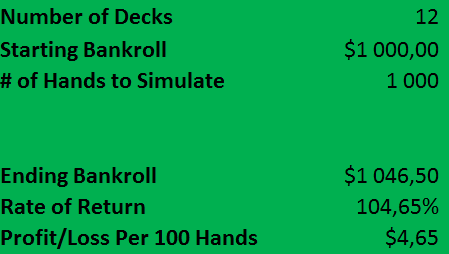
\includegraphics[scale=0.37]{BasicAAngepastGoedResultaat.png}
%    \caption{goed resultaat}
%\end{figure}
\begin{table}[htbp]
\caption{Goed resultaat}
\tiny
\centering
\begin{tabular}{|
>{}l 
>{}r |}
\hline
\multicolumn{1}{|l|}{Number of decks} & 12 \\ \hline
\multicolumn{1}{|l|}{Starting bankroll} & \$1000,00 \\ \hline
\multicolumn{1}{|l|}{\# of hands to simulate} & 1000 \\ \hline
 &  \\ \hline
\multicolumn{1}{|l|}{Ending bankroll} & \$1046,50 \\ \hline
\multicolumn{1}{|l|}{Rate return} & 104,65\% \\ \hline
\multicolumn{1}{|l|}{\Profit/Loss per 100 hands} & \$4,65 \\ \hline
\end{tabular}
\end{table}



 
Maar na meerdere simulaties hebben we kunnen zien dat het resultaat inconsistent is. En dat er grote verschillen zaten tussen het beste en slechtste resultaat. Zo hebben wij een schommeling van 30 euro kunnen waarnemen. In tegenstelling tot de orgineële versie waar de schommeling beperkt is gebleven tot 10 euro tegenover het gemiddelde. Het is dan ook door dit verschil tussen het beste en slechtste resultaat dat onze strategie minder aantrekkelijk maakt. We hebben dan ook kunnen besluiten dat het niet mogelijk is om deze strategie te verbeteren en daarbij een consistent resultaat te verkrijgen.
%\begin{figure}[hb]
%    \centering
%    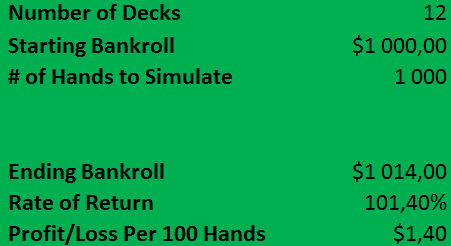
\includegraphics[scale=0.37]{BasicAangepastSlechtsteResultaat.png}
%    \caption{Slecht resultaat}
%\end{figure}
\begin{table}[htbp]
\caption{Slecht resultaat}
\tiny
\centering
\begin{tabular}{|
>{}l 
>{}r |}
\hline
\multicolumn{1}{|l|}{Number of decks} & 12 \\ \hline
\multicolumn{1}{|l|}{Starting bankroll} & \$1000,00 \\ \hline
\multicolumn{1}{|l|}{\# of hands to simulate} & 1000 \\ \hline
 &  \\ \hline
\multicolumn{1}{|l|}{Ending bankroll} & \$1014,00 \\ \hline
\multicolumn{1}{|l|}{Rate return} & 101,40\% \\ \hline
\multicolumn{1}{|l|}{Profit/Loss per 100 hands} & \$1,40 \\ \hline
\end{tabular}
\end{table}
\begin{table}[htbp]
\setlength{\tabcolsep}{3pt}
\caption{Aangepaste basic strategie}
\tiny
\centering
\begin{tabular}{|c|c|c|c|c|c|c|c|c|c|c|}
\hline
 & \multicolumn{10}{c|}{\textbf{Dealer's face-up card}} \\ \cline{2-11} 
\multirow{-2}{*}{\textbf{\begin{tabular}[c]{@{}c@{}}Player\\ hand\end{tabular}}} & \textbf{2} & \textbf{3} & \textbf{4} & \textbf{5} & \textbf{6} & \textbf{7} & \textbf{8} & \textbf{9} & \textbf{10} & \textbf{11} \\ \hline
\multicolumn{11}{|c|}{\textbf{Hard totals (excluding pairs)}} \\ \hline
\textbf{21} & \cellcolor[HTML]{32CB00}S & \cellcolor[HTML]{32CB00}S & \cellcolor[HTML]{32CB00}S & \cellcolor[HTML]{32CB00}S & \cellcolor[HTML]{32CB00}S & \cellcolor[HTML]{32CB00}S & \cellcolor[HTML]{32CB00}S & \cellcolor[HTML]{32CB00}S & \cellcolor[HTML]{32CB00}S & \cellcolor[HTML]{32CB00}S \\ \hline
\textbf{12} & \cellcolor[HTML]{FE0000}H & \cellcolor[HTML]{FE0000}H & \cellcolor[HTML]{FE0000}H & \cellcolor[HTML]{FE0000}H & \cellcolor[HTML]{FE0000}H & \cellcolor[HTML]{FE0000}H & \cellcolor[HTML]{FE0000}H & \cellcolor[HTML]{FE0000}H & \cellcolor[HTML]{FE0000}H & \cellcolor[HTML]{FE0000}H \\ \hline

\end{tabular}
\end{table}


\subsubsection{Perfect strategie}
Sinds deze strategie een verder gevorde strategie is van de basic hebben we hier met dezelfde aanpassingen gewerkt als bij de vorige. Hier zagen we snel dat deze strategie niet verbeterd kon worden omdat de winstmarge van de aangepaste versie gemiddeld 10 euro minder was dan die van de orginele. We zagen ook bij het gemiddelde dat hier de winst veel lager lag dan bij de orginele strategie. Dit komt om dat deze strategie een verder gevorde versie is van de basic en dus ook beter uitgewerkt. Dit zorgde er dan ook voor dat deze versie direct werd afgekeurd.  
\begin{table}[htbp]
\setlength{\tabcolsep}{3pt}
\caption{Aangepaste rij in perfect strategie}
\tiny
\centering
\begin{tabular}{|c|c|c|c|c|c|c|c|c|c|c|}
\hline
 & \multicolumn{10}{c|}{\textbf{Dealer's face-up card}} \\ \cline{2-11} 
\multirow{-2}{*}{\textbf{\begin{tabular}[c]{@{}c@{}}Player\\ hand\end{tabular}}} & \textbf{2} & \textbf{3} & \textbf{4} & \textbf{5} & \textbf{6} & \textbf{7} & \textbf{8} & \textbf{9} & \textbf{10} & \textbf{11} \\ \hline
\multicolumn{11}{|c|}{\textbf{Hard totals (excluding pairs)}} \\ \hline
\textbf{12} & \cellcolor[HTML]{FE0000}H & \cellcolor[HTML]{FE0000}H & \cellcolor[HTML]{FE0000}H & \cellcolor[HTML]{FE0000}H & \cellcolor[HTML]{FE0000}H & \cellcolor[HTML]{FE0000}H & \cellcolor[HTML]{FE0000}H & \cellcolor[HTML]{FE0000}H & \cellcolor[HTML]{FE0000}H & \cellcolor[HTML]{FE0000}H \\ \hline
\end{tabular}
\end{table}


\subsection{ Waar zal voor elke strategie de kans op winst stagneren, waar ligt het optimale punt van die bepaalde strategie?}
Voor beide strategieën is het wel duidelijk dat de kans op winst vergroot als het aantal gespeelde rondes verhoogd, we zien  dat bij 100 rondes er nog altijd verlies kan gemaakt worden omdat het ook nog altijd afhangt van de kaarten die de speler en de dealer krijgt  maar als we dan meer rondes beginnen te spelen zoals 1000 kunnen we wel zien dat er winst begint te komen Hierdoor kunnen we zeggen dat de resultaten wel lichtjes beïnvloedbaar zijn maar dat men daar een groot aantal rondes voor moet spelen eer het resultaat zichtbaar wordt en er zekerheid is. Er moet ook rekening gehouden worden dat deze strategie\"{e}n goed zijn om gebruiken maar dat men ook nog rekening moet houden met de kaarten die zichtbaar zijn. Zo hebben we gezien dat iemand die alleen de strategie toepast zonder rekening te houden met de kaarten vaker verliest dan iemand die de kaarten telt en deze strategie\"{e}n gaat toe passen.

\section{Toepassen van analyse op 1 variabele}
\subsection{Basic strategie}

\begin{table}[htbp]
\caption{Analyse - Basic strategie}
\tiny
\centering
\begin{tabular}{|l|lll}
\cline{1-1} \cline{3-4}
\textbf{Waarnemingen:} & \multicolumn{1}{l|}{} & \multicolumn{1}{l|}{\textbf{Median:}} & \multicolumn{1}{l|}{1039,75} \\ \cline{1-1} \cline{3-4} 
1039,5 & \multicolumn{1}{l|}{} & \multicolumn{1}{l|}{\textbf{Modus:}} & \multicolumn{1}{l|}{1042} \\ \cline{1-1} \cline{3-4} 
1045 & \multicolumn{1}{l|}{} & \multicolumn{1}{l|}{\textbf{Bereik:}} & \multicolumn{1}{l|}{16,5} \\ \cline{1-1} \cline{3-4} 
1032,5 & \multicolumn{1}{l|}{} & \multicolumn{1}{l|}{\textbf{Q1:}} & \multicolumn{1}{l|}{1035,5} \\ \cline{1-1} \cline{3-4} 
1040 & \multicolumn{1}{l|}{} & \multicolumn{1}{l|}{\textbf{Q2:}} & \multicolumn{1}{l|}{1039,75} \\ \cline{1-1} \cline{3-4} 
1042 & \multicolumn{1}{l|}{} & \multicolumn{1}{l|}{\textbf{Q3:}} & \multicolumn{1}{l|}{1042} \\ \cline{1-1} \cline{3-4} 
1034,5 & \multicolumn{1}{l|}{} & \multicolumn{1}{l|}{\textbf{Variantie:}} & \multicolumn{1}{l|}{23,3525} \\ \cline{1-1} \cline{3-4} 
1035 & \multicolumn{1}{l|}{} & \multicolumn{1}{l|}{\textbf{Standaardafwijking:}} & \multicolumn{1}{l|}{4,832442} \\ \cline{1-1} \cline{3-4} 
1042 & \multicolumn{1}{l|}{} & \multicolumn{1}{l|}{\textbf{Gemidelde:}} & \multicolumn{1}{l|}{1039,65} \\ \cline{1-1} \cline{3-4} 
1037 &  &  &  \\ \cline{1-1}
1049 &  & \textbf{} &  \\ \cline{1-1}
\end{tabular}
\end{table}

\subsection{Perfect strategie}

\begin{table}[htbp]
\caption{Analyse - Perfect strategie}
\tiny
\centering
\begin{tabular}{|l|lll}
\cline{1-1} \cline{3-4}
\textbf{Waarnemingen:} & \multicolumn{1}{l|}{} & \multicolumn{1}{l|}{\textbf{Median:}} & \multicolumn{1}{l|}{1024,5} \\ \cline{1-1} \cline{3-4} 
1031,5 & \multicolumn{1}{l|}{} & \multicolumn{1}{l|}{\textbf{Modus:}} & \multicolumn{1}{l|}{1016} \\ \cline{1-1} \cline{3-4} 
1037 & \multicolumn{1}{l|}{} & \multicolumn{1}{l|}{\textbf{Bereik:}} & \multicolumn{1}{l|}{39} \\ \cline{1-1} \cline{3-4} 
1018 & \multicolumn{1}{l|}{} & \multicolumn{1}{l|}{\textbf{Q1:}} & \multicolumn{1}{l|}{1016,5} \\ \cline{1-1} \cline{3-4} 
1048,5 & \multicolumn{1}{l|}{} & \multicolumn{1}{l|}{\textbf{Q2:}} & \multicolumn{1}{l|}{1024,5} \\ \cline{1-1} \cline{3-4} 
1042 & \multicolumn{1}{l|}{} & \multicolumn{1}{l|}{\textbf{Q3:}} & \multicolumn{1}{l|}{1035,625} \\ \cline{1-1} \cline{3-4} 
1021,5 & \multicolumn{1}{l|}{} & \multicolumn{1}{l|}{\textbf{Variantie:}} & \multicolumn{1}{l|}{146,6625} \\ \cline{1-1} \cline{3-4} 
1016 & \multicolumn{1}{l|}{} & \multicolumn{1}{l|}{\textbf{Standaardafwijking:}} & \multicolumn{1}{l|}{12,110429} \\ \cline{1-1} \cline{3-4} 
1009,5 & \multicolumn{1}{l|}{} & \multicolumn{1}{l|}{\textbf{Gemidelde:}} & \multicolumn{1}{l|}{1026,75} \\ \cline{1-1} \cline{3-4} 
1027,5 &  &  &  \\ \cline{1-1}
1016 &  & \textbf{} &  \\ \cline{1-1}
\end{tabular}
\end{table}

\section{Conclusie}
Ook al kunnen deze strategie\"{e}n de speler een voordeel geven tegenover de dealer toch is het nog altijd geen zekerheid dat men winst kan maken. Om de kans nog te vergroten moet de strategie\"{e}n toegepast worden samen met andere technieken zoals het tellen van kaarten. Maar nog  weten we niet alle variabelen die worden gebruikt in een casino. We kunnen dus concluderen dat all deze methodes de kansen wel zullen vergroten maar dat de kansen nog altijd in het voordeel van de casino's zullen zijn.

\section*{Erkenning}

We zouden graag alle auteurs willen bedanken van de bronnen die we hebben gebruikt en ook de maker van onze excel simulator die we hebben gevonden op het internet. Ook zouden we onze docent willen bedanken voor het helpen bij het vinden van een goede onderzoeksvraag.
\nocite{*}

\bibliographystyle{IEEEtran}
\bibliography{Bronnen}


\end{document}
